% Replicator dynamics: the room as a population playing the snowdrift game.
% Shared preamble for the write-on class slides.
%
% Every deck is designed to be projected and annotated live on a tablet:
% whatever takes time to draw is pre-drawn, and whatever the class produces is
% left blank. Compile a deck with `pdflatex main.tex` from its own directory,
% or run `make` in decks/ to build them all.
\documentclass[10pt]{article}

\usepackage[papersize={25.6cm,14.4cm}, margin=1.1cm, bottom=1.5cm,
            footskip=0.75cm]{geometry}
\usepackage[T1]{fontenc}
\usepackage[default]{sourcesanspro}
\usepackage{newtxsf}
\usepackage{tikz}
\usepackage{amsmath}
\usepackage{parskip}
\usepackage{fancyhdr}
\usetikzlibrary{arrows.meta, positioning, calc}

\setlength{\parindent}{0pt}

% Catppuccin Latte, the palette the course site uses in its light theme, so a
% deck on the projector looks like the pages the students read.
\definecolor{inkbg}{HTML}{EFF1F5}      % base
\definecolor{inksurface}{HTML}{E6E9EF} % mantle
\definecolor{inkfaint}{HTML}{CCD0DA}   % surface2, for rules and empty boxes
\definecolor{inktext}{HTML}{4C4F69}    % text
\definecolor{inkgrey}{HTML}{8C8FA1}    % overlay1, for anything secondary
\definecolor{inkblue}{HTML}{7287FD}    % lavender, the primary accent
\definecolor{inkteal}{HTML}{179299}    % teal
\definecolor{inkred}{HTML}{FE640B}     % peach, for whatever wants attention
\definecolor{inkmauve}{HTML}{8839EF}   % mauve

\pagecolor{inkbg}
\color{inktext}

% A box to write a number into. White against the tinted page, so it reads as
% somewhere to write rather than as part of the printed material.
\newcommand{\blank}[1][1.6]{%
  \tikz[baseline=(current bounding box.base)]{%
    \draw[inkfaint, line width=0.7pt, rounded corners=2pt, fill=white]
      (0,-0.18) rectangle (#1,0.62);}}

% A ruled area to work in. Faint dots keep handwriting level on a tablet.
\newcommand{\workspace}[2]{%
  \begin{tikzpicture}
    \draw[inkfaint, line width=0.7pt, rounded corners=3pt, fill=white]
      (0,0) rectangle (#1,#2);
    \foreach \gx in {0.5,1.0,...,#1}{%
      \foreach \gy in {0.5,1.0,...,#2}{%
        \fill[inkfaint] (\gx,\gy) circle (0.5pt);}}
  \end{tikzpicture}}

% A panel for material that is printed rather than written on.
\newcommand{\panel}[2]{%
  \begin{tikzpicture}
    \draw[inkfaint, line width=0.7pt, rounded corners=3pt, fill=inksurface]
      (0,0) rectangle (#1,#2);
  \end{tikzpicture}}

% An empty payoff grid. #1 is the list of action names, #2 is drawn afterwards
% so a page can add its own marks.
\newcommand{\payoffgrid}[2]{%
  \begin{tikzpicture}[scale=1.0, every node/.style={transform shape}]
    \foreach \name [count=\j from 0] in {#1}{%
      \node[font=\bfseries, text=inkblue] at (\j*2.7+1.35,0.55) {\name};
      \node[font=\bfseries, text=inkblue] at (-1.15,-\j*2-1) {\name};
      \foreach \k [count=\i from 0] in {#1}{%
        \draw[inkfaint, line width=0.7pt, fill=white]
          (\j*2.7,-\i*2) rectangle (\j*2.7+2.7,-\i*2-2);}}
    #2
  \end{tikzpicture}}

% The five actions on a pentagon. Each action beats the one next to it and the
% one across from it, so the two winning cycles are drawn as separate panels:
% ten labelled arrows on one diagram is a tangle nobody can read from the back
% of the room.
\newcommand{\rpslscycle}[3]{%
  \begin{tikzpicture}[scale=1.0, every node/.style={transform shape},
      >={Stealth[length=2.6mm]},
      action/.style={circle, draw=inkfaint, line width=1pt, fill=white,
                     text=inktext, minimum size=1.7cm, inner sep=1pt,
                     font=\small\bfseries},
      beats/.style={->, line width=1.2pt, shorten >=3pt, shorten <=3pt,
                    draw=#1},
      word/.style={font=\scriptsize, fill=inkbg, inner sep=1.6pt, text=#1,
                   sloped, pos=#2}]
    \foreach \name/\angle in {Rock/90, Lizard/18, Spock/-54,
                              Scissors/-126, Paper/162}{%
      \node[action] (\name) at (\angle:3.1) {\name};}
    \foreach \winner/\loser/\said in {#3}{%
      \draw[beats] (\winner) -- node[word] {\said} (\loser);}
  \end{tikzpicture}}

% Running header: the deck name on the left, the page's own step on the right.
% Each deck sets its name once with \deckname.
\newcommand{\deck}{}
\newcommand{\deckname}[1]{\renewcommand{\deck}{#1}}
\newcommand{\slidehead}[1]{%
  {\small\color{inkgrey}%
   \tikz[baseline=-0.5ex]{\fill[inkblue, rounded corners=1pt]
     (0,0) rectangle (0.22,0.22);}\;\deck
   \hfill \color{inkblue}\bfseries #1}\par
  {\color{inkblue}\rule{\linewidth}{1pt}}\par\vspace{0.35em}}

\pagestyle{fancy}
\fancyhf{}
\renewcommand{\headrulewidth}{0pt}
\fancyfoot[R]{\small\color{inkgrey}\thepage}

% Deck title pages, which carry no header and no page number.
\newcommand{\titleslide}[3]{%
  \thispagestyle{empty}%
  \begin{center}
    \vspace*{\fill}
    {\Huge\bfseries\color{inkblue} #1}\\[0.7em]
    {\LARGE\color{inkgrey} #2}\\[2.4em]
    #3
    \vspace*{\fill}
  \end{center}}

% One step of the plan on a title page.
\newcommand{\stepbox}[3]{%
  \node[draw=inkblue, line width=0.9pt, rounded corners=4pt, fill=white,
        minimum width=6cm, minimum height=1.7cm, align=center,
        text=inktext] (#1) at (#2,0) {#3};}


% Blank axes for plotting the fraction on the Dig side, round by round.
\newcommand{\trajectory}{%
  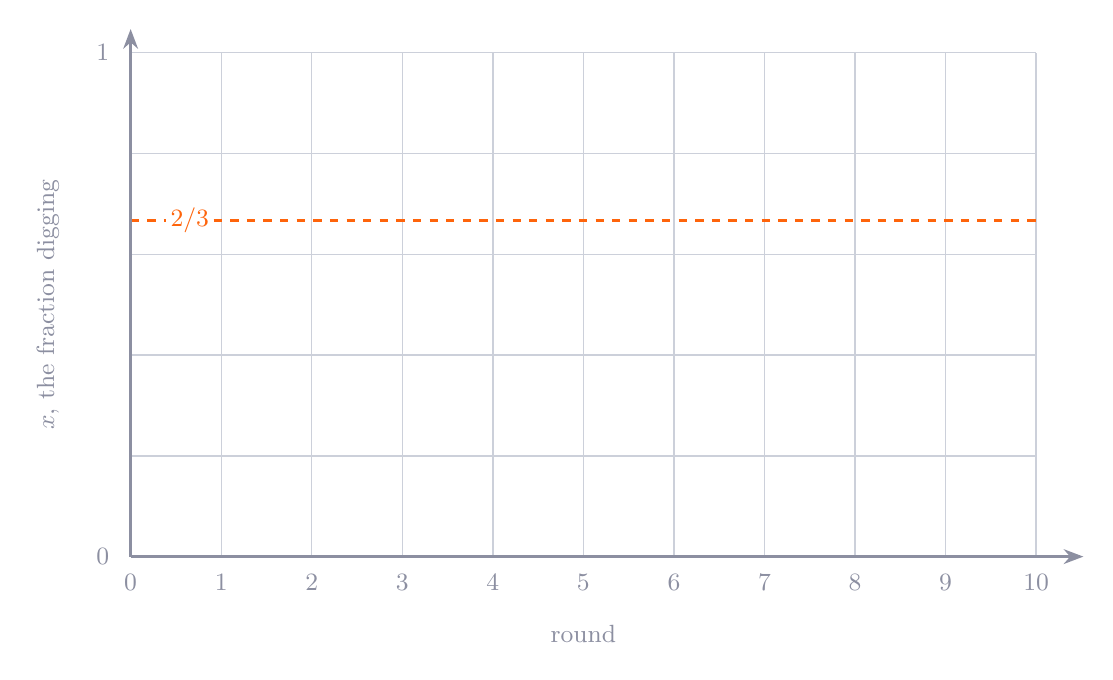
\begin{tikzpicture}[scale=1.0, every node/.style={transform shape}]
    \fill[white] (0,0) rectangle (11.5,6.4);
    \foreach \r in {0,1,...,10}{%
      \draw[inkfaint, line width=0.5pt] (\r*1.15,0) -- (\r*1.15,6.4);
      \node[below, font=\small, text=inkgrey] at (\r*1.15,-0.1) {\r};}
    \foreach \y in {0,1,...,5}{%
      \draw[inkfaint, line width=0.5pt] (0,\y*1.28) -- (11.5,\y*1.28);}
    \draw[inkred, line width=1pt, dashed] (0,4.267) -- (11.5,4.267);
    \node[font=\small, text=inkred, fill=white, inner sep=1.5pt]
      at (0.75,4.267) {$2/3$};
    \draw[inkgrey, line width=1pt, -{Stealth[length=2.5mm]}] (0,0) -- (12.1,0);
    \draw[inkgrey, line width=1pt, -{Stealth[length=2.5mm]}] (0,0) -- (0,6.7);
    \node[left, font=\small, text=inkgrey] at (-0.15,0) {$0$};
    \node[left, font=\small, text=inkgrey] at (-0.15,6.4) {$1$};
    \node[below, font=\small, text=inkgrey] at (5.75,-0.75) {round};
    \node[font=\small, text=inkgrey, rotate=90] at (-1.05,3.2)
      {$x$, the fraction digging};
  \end{tikzpicture}}

\deckname{Replicator dynamics}

\begin{document}

\titleslide{Replicator dynamics}{The room is the population}{%
    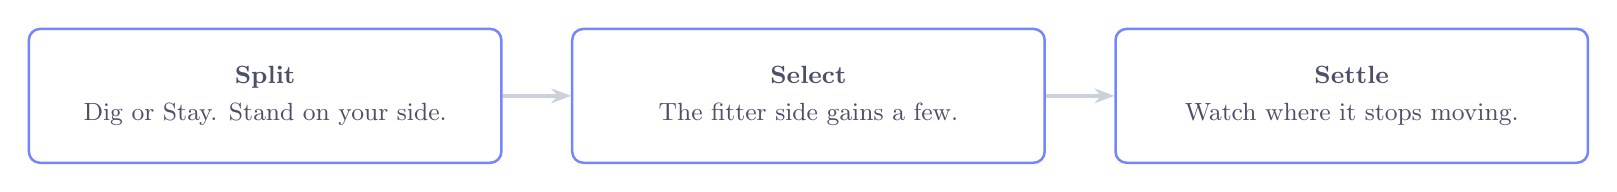
\begin{tikzpicture}[font=\small]
      \stepbox{s0}{0.0}{\textbf{Split}\\[0.25em]
        Dig or Stay. Stand on your side.}
      \stepbox{s1}{6.9}{\textbf{Select}\\[0.25em]
        The fitter side gains a few.}
      \stepbox{s2}{13.8}{\textbf{Settle}\\[0.25em]
        Watch where it stops moving.}
      \draw[-{Stealth[length=2.5mm]}, inkfaint, line width=1.2pt] (s0) -- (s1);
      \draw[-{Stealth[length=2.5mm]}, inkfaint, line width=1.2pt] (s1) -- (s2);
    \end{tikzpicture}

    \vspace{2.4em}

    {\large In the room: \blank[2.2] \hspace{2cm}
     Starting split: \blank[2.2] digging}}

\newpage
\slidehead{The snowdrift}

\vspace{0.2cm}

\begin{minipage}[c]{0.46\linewidth}
\begin{center}
\payoffgrid{Dig, Stay}{%
  \node at (1.35,-1) {\Large $3$};
  \node at (4.05,-1) {\Large $2$};
  \node at (1.35,-3) {\Large $4$};
  \node at (4.05,-3) {\Large $0$};}
\end{center}
\end{minipage}
\hfill
\begin{minipage}[c]{0.50\linewidth}
\raggedright
{\large Clearing the drift is worth 4 to each of you. Digging costs 2, shared
if you both dig.}

\vspace{1.2em}

{\large Two diggers get 3 each. A lone digger gets \blank[1.4] while the
other free-rides for \blank[1.4]. Two stayers get \blank[1.4].}

\vspace{1.2em}

{\large Would you rather be the one digging? \blank[2.2]}
\end{minipage}

\newpage
\slidehead{Round by round}

\vspace{0.1cm}

\begin{minipage}[c]{0.60\linewidth}
\trajectory
\end{minipage}
\hfill
\begin{minipage}[c]{0.36\linewidth}
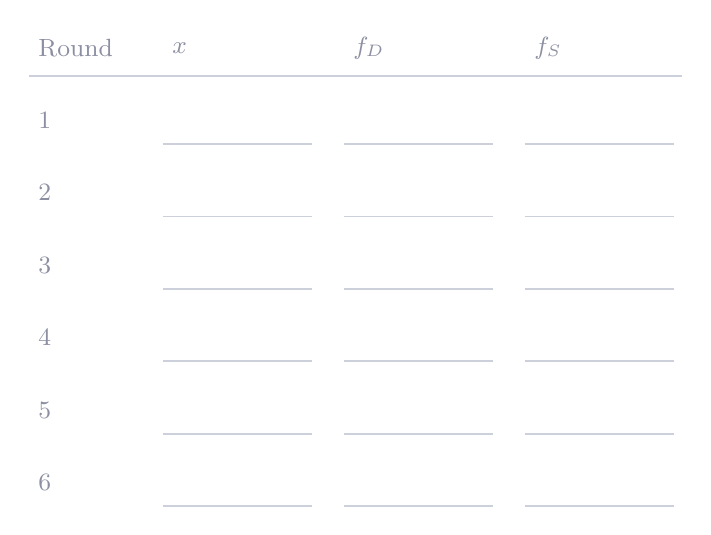
\begin{tikzpicture}[font=\small]
  \foreach \lab/\col in {Round/0, $x$/1.7, $f_D$/4.0, $f_S$/6.3}{%
    \node[anchor=west, text=inkgrey] at (\col,0) {\lab};}
  \draw[inkfaint, line width=0.7pt] (0,-0.36) -- (8.3,-0.36);
  \foreach \row in {1,2,3,4,5,6}{%
    \node[anchor=west, text=inkgrey] at (0,-0.92*\row) {\row};
    \foreach \col in {1.7,4.0,6.3}{%
      \draw[inkfaint, line width=0.7pt]
        (\col,-0.92*\row-0.3) -- (\col+1.9,-0.92*\row-0.3);}}
\end{tikzpicture}
\end{minipage}

\vspace{0.3cm}

{\small\color{inkgrey} Plot the split each round. The dashed line is where we
expect it to end up.}

\newpage
\slidehead{Which side is doing better?}

\vspace{0.8cm}

{\large With a fraction \(x\) digging,}

\vspace{0.7cm}

\begin{center}
{\Large \(f_D \;=\;\) \blank[5.4] \hspace{2.4cm} \(f_S \;=\;\) \blank[5.4]}
\end{center}

\vspace{1.2cm}

{\large They are equal when \(x =\) \blank[2], which is where the room
\underline{\hspace{4cm}}.}

\vspace{1cm}

\begin{center}
\workspace{22.6}{3}
\end{center}

\newpage
\slidehead{Turning the room into an equation}

\vspace{0.7cm}

{\large A strategy grows when it does better than the population average
\(\phi = x f_D + (1 - x) f_S\). How fast it grows depends on two things:}

\vspace{0.9cm}

\hspace{1cm}

\begin{tikzpicture}[font=\large]
  \node[anchor=west] at (0,0)
    {how far above average it is: \blank[3.4]};
  \node[anchor=west] at (11.6,0)
    {and how many already play it: \blank[3.4]};
\end{tikzpicture}

\vspace{1.2cm}

\begin{center}
{\Huge \(\dot{x} \;=\;\) \blank[6]}
\end{center}

\vspace{1.2cm}

{\large Each round of the activity, with its small fixed step, was one step of
\underline{\hspace{5cm}} on this equation.}

\newpage
\slidehead{Where it can rest, and where it goes}

\vspace{0.6cm}

{\large Factorise \(\dot{x}\) and read off every value where it is zero:}

\vspace{0.6cm}

\begin{center}
\workspace{22.6}{3.6}
\end{center}

\vspace{0.8cm}

{\large Rest points: \blank[2] \hspace{1.2cm} \blank[2] \hspace{1.2cm}
\blank[2]}

\vspace{0.9cm}

{\large For \(0 < x < 2/3\) the sign of \(\dot{x}\) is \blank[1.4], and for
\(2/3 < x < 1\) it is \blank[1.4]. So from anywhere inside, the population
moves towards \blank[2].}

\newpage
\slidehead{Is it evolutionarily stable?}

\vspace{0.9cm}

{\large A small group of Stayers invades a population sitting at
\(x = 2/3\). Do they earn more or less than the residents? \blank[3]}

\vspace{1.2cm}

\begin{center}
\workspace{22.6}{4}
\end{center}

\vspace{1cm}

{\large So \(x = 2/3\) \underline{\hspace{3cm}} an ESS. Rock-Paper-Scissors
has an interior rest point too, but there the dynamics
\underline{\hspace{4cm}} instead of settling.}

\newpage
\slidehead{The same thing, as an exam answer}

\vspace{0.5cm}

{\large What we just did in the room is \textbf{Question 1} on the Replicator
Dynamics page.}

\vspace{0.9cm}

\hspace{0.6cm}
\begin{minipage}{0.92\linewidth}
{\large
\begin{tabbing}
\hspace{1.2cm} \= \hspace{17cm} \= \kill
\textbf{(a)} \> The fitnesses \(f_D\) and \(f_S\) as functions of
  \(x\). \> [3]\\[0.55em]
\textbf{(b)} \> The replicator equation, simplified to a product of
  factors. \> [7]\\[0.55em]
\textbf{(c)} \> All stable populations. \> [3]\\[0.55em]
\textbf{(d)} \> From the sign of \(\dot{x}\), which one we approach, and where
  the class settled. \> [6]\\[0.55em]
\textbf{(e)} \> Whether the interior population is an ESS, argued two
  ways. \> [6]
\end{tabbing}}
\end{minipage}

\vspace{1.2cm}

\begin{center}
{\large\color{inkgrey} vknight.org/gt/topics/replicator-dynamics.html}
\end{center}

\end{document}
